\subsection*{Introduction}

The Midori64 block cipher is a lightweight substitution-permutation network
(SPN) cipher, designed with a focus on simplicity and security. The MILP model
for Midori64 aims to study and optimize the differential characteristics of the
cipher. This model captures the linear constraints for the cipher's round
operations, such as the non-linear S-box function, cell shuffling, and column
mixing, to calculate the minimal number of active S-boxes. The model uses the
concept of convex hulls to describe the relationship between the input and
output differences, which simplifies the analysis and computation.

The MILP model can be divided into three primary operations, each described by
its set of constraints.


\subsection{Substitution Cell Operation}

The substitution cell involves a transformation from the input variables \(
x_i^j \) to the output variables \( y_i^j \) through a substitution box (S-box  $a_i^j$ ).
The key components are as follows:

\begin{itemize}
    \item \( x_i^j \): Binary input variables where \( i \) is the round number
          and \( j \) is the variable index (ranging from 0 to 63).
    \item \( a_i^j \): Binary variable indicating whether the S-box \( j \) is
          active in round \( i \).
    \item \( p_i^j_k \): Probability binary variables for each S-box and each
          input-output pair, where \( k \) can take values 0 or 1.
    \item \( y_i^j \): Binary output variables where \( i \) is the round number and \( j \) is the variable index (ranging from 0 to 63).
\end{itemize}

% \begin{center}
% 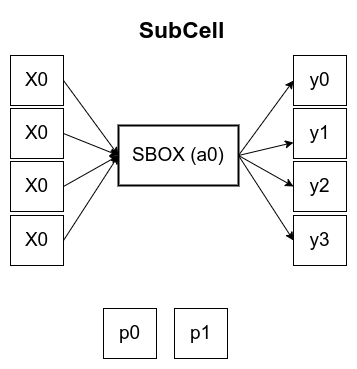
\includegraphics[width=5.5cm]{../images/subcell.png}
% \end{center}

The transformation is done through a set of constraints for each nibble (group
of 4 input/output variables) of the substitution.

\subsection*{Constraints}

For each nibble of input \( x_{i,0}, x_{i,1}, x_{i,2}, x_{i,3} \) and output \( y_{i,0}, y_{i,1}, y_{i,2}, y_{i,3} \), the following constraints are applied:

\begin{align*}
    x_{i,0} - a_{i,0}                                                                  & \leq 0 \\
    x_{i,1} - a_{i,0}                                                                  & \leq 0 \\
    x_{i,2} - a_{i,0}                                                                  & \leq 0 \\
    x_{i,3} - a_{i,0}                                                                  & \leq 0 \\
    x_{i,0} + x_{i,1} + x_{i,2} + x_{i,3} - a_{i,0}                                    & \geq 0 \\
    4(x_{i,0} + x_{i,1} + x_{i,2} + x_{i,3}) - (y_{i,0} + y_{i,1} + y_{i,2} + y_{i,3}) & \geq 0 \\
    4(y_{i,0} + y_{i,1} + y_{i,2} + y_{i,3}) - (x_{i,0} + x_{i,1} + x_{i,2} + x_{i,3}) & \geq 0
\end{align*}


\begin{itemize}
    \item \( \highlightmath{x_{i,j} - a_{i,j} \leq 0} \):
          This constraint ensures that the values of \(x_{i,j}\) do not exceed the threshold represented by \(a_{i,j}\). It limits the possible states of \(x_{i,j}\), preventing values of \(x_{i,j}\) from surpassing the allowable range determined by \(a_{i,j}\).

    \item \(\highlightmath{x_{i,0} + x_{i,1} + x_{i,2} + x_{i,3} - a_{i,0} \geq 0}\):
          This constraint ensures that the sum of the elements in the first nibble of \(x_i\) (i.e., \(x_{i,0}, x_{i,1}, x_{i,2}, x_{i,3}\)) is greater than or equal to the threshold value \(a_{i,0}\). It eliminates combinations where the total value of \(x_i\) is too small, ensuring it meets the minimum threshold.

    \item \(\highlightmath{4(x_{i,0} + x_{i,1} + x_{i,2} + x_{i,3}) - (y_{i,0} + y_{i,1} + y_{i,2} + y_{i,3}) \geq 0}\):
          This constraint ensures that four times the sum of the values in \(x_i\) is always greater than or equal to the sum of the corresponding values in \(y_i\). It removes invalid combinations where the values of \(y_i\) could exceed the scaled value of \(x_i\), maintaining a consistent relationship between the variables.

    \item \(\highlightmath{4(y_{i,0} + y_{i,1} + y_{i,2} + y_{i,3}) - (x_{i,0} + x_{i,1} + x_{i,2} + x_{i,3}) \geq 0}\):
          This constraint does the reverse of the previous one, ensuring that the scaled sum of the values in \(y_i\) is greater than or equal to the sum of the corresponding values in \(x_i\). It eliminates combinations where the \(x_i\) values could overpower the \(y_i\) values, ensuring balance and validity between the two.

\end{itemize}


\subsection*{Differential Distribution Table (DDT) and Convex Hull}

The Differential Distribution Table (DDT) is used to describe the probability
distribution of differences in the output (delta-out) for given differences in
the input (delta-in). This table helps to identify impossible transition from
form input to \texttt{Sbox} and it's output from \texttt{Sbox}.

\subsection*{Convex Hull and its Role}
The concept of a convex hull plays a significant role in optimizing the
inequalities generated by the DDT. A convex hull is the smallest convex set that
contains a set of points, and it helps in defining the feasible region for the
inequalities.

By using the convex hull, we can construct a set of inequalities that represent
the feasible region for the DDT. These inequalities will help in constraining
the possible output patterns, thus making help to find differential possible pattern by
eliminating impossible patterns.

\begin{center}
    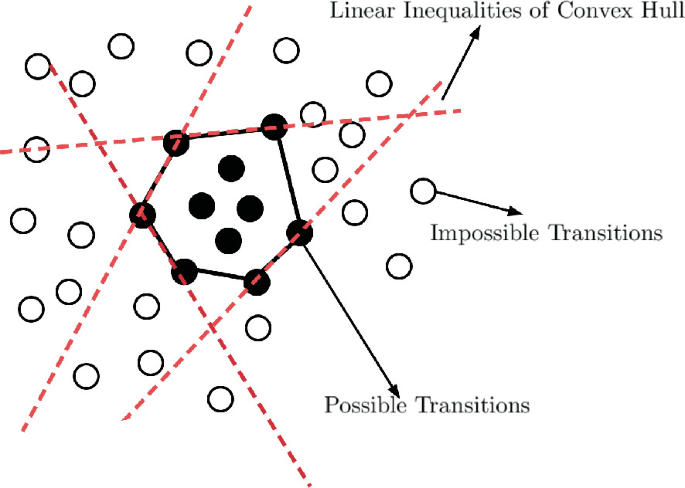
\includegraphics[width=10cm]{./images/convex_hull.png}
\end{center}

\subsection*{Constructing Parameters and Inequalities}
\begin{itemize}
    \item We first generate the DDT, which describes how changes in the input affect the output of the S-box.
    \item Next, we identify the possible and impossible points based on the DDT.
          The possible points represent valid input-output pairs with non-zero
          probabilities.
    \item Using the convex hull, we generate inequalities that describe the
          feasible region of the DDT.
    \item Each inequality defines a region of valid patterns that satisfy the
          constraints imposed by the SubCell transformation.
\end{itemize}

\subsection*{Generating 239 Inequalities Using Convex Hull}
To generate all 239 inequalities for the Sigle SBox from transformation, we
first construct a polyhedron using the convex hull of the possible points. Then,
we extract the inequalities from the polyhedron representation. This step
provides a comprehensive set of constraints that define the valid regions of the
DDT.

\begin{align*}
    \text{Convex Hull Constraints:} \quad \sum_{i=1}^{n} \text{coeff}_i \cdot x_i + b \geq 0 \\
    x_i = (x_0,x_1,x_2,x_3,y_0,y_1,y_2,y_3,p_0,p_1)
\end{align*}
and mapping for the $p_i$ to probabilities from DDT is as follows

\begin{center}
    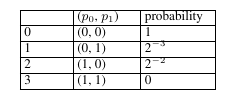
\includegraphics[width=5.5cm]{./images/table.png}
\end{center}

This inequality represents the constraints for each region of the convex hull,
where the coefficients \( \text{coeff}_i \) and the constant \( b \) are derived
from the convex hull construction.

\subsection*{Greedy Algorithm to Reduce Constraints}
Once the convex hull has been constructed, the next step is to reduce the number
of constraints. This is done using a greedy algorithm that selects the most
effective inequalities to keep while discarding redundant ones. The greedy
algorithm iteratively removes inequalities that do not significantly reduce the
feasible region.

The algorithm works by comparing the number of impossible points that each
inequality removes. The best inequality is selected, and the process continues
until a reduced set of constraints is achieved.

The Python code for this process is provided below:

\begin{lstlisting}[language=Python]
def reduce_inequalites(inequalities, impossible_points):
    reduced_set = set()

    while impossible_points:
        best_inequality = None
        max_removed_patterns = 0

        for inequality in inequalities:
            removed_patterns = removed_impossible_patterns(
                inequality, impossible_points)

            if len(removed_patterns) > max_removed_patterns:
                max_removed_patterns = len(removed_patterns)
                best_inequality = inequality

        if best_inequality is not None:
            removed_patterns = removed_impossible_patterns(
                best_inequality, impossible_points)

            impossible_points = [point for point in impossible_points 
                                 if point not in removed_patterns]
            reduced_set.add(best_inequality)
            inequalities.remove(best_inequality)

    return reduced_set
\end{lstlisting}

This code effectively reduces the number of inequalities from 239 to 26 by
selecting the most impactful constraints for Differential Distribution Table (DDT).
These 26 Constraints are as follows:
\begin{center}
    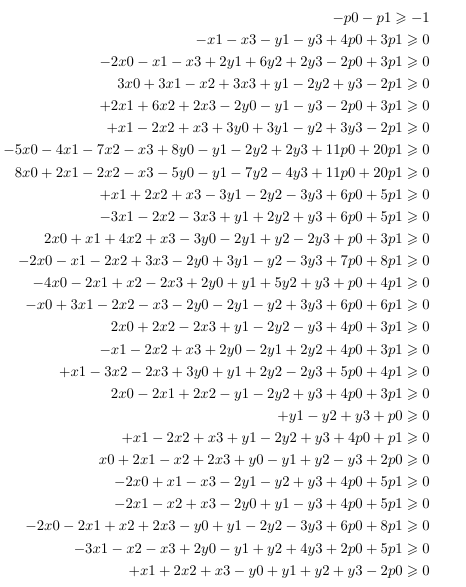
\includegraphics[width=10cm]{./images/sbox_equations.png}
\end{center}

This pattern repeats for all 16 S-boxes (from \( a_0 \) to \( a_{15} \)) in a
single round \( i \).


\subsection{Suffle Cell Operation}

The \textbf{ShuffleCell} operation ensures diffusion by shuffling the input values (\( y_{i,j} \)) into
new positions to produce the output values (\( z_{i,j} \)).

\textbf{Transformation Rules}

\[
    (z_0, z_1, z_2, \ldots, z_{15}) \leftarrow (y_0, y_{10}, y_5, y_{15}, y_{14}, y_{4}, y_{11}, y_{1}, y_{9}, y_{3}, y_{12}, y_{6}, y_{7}, y_{13}, y_{2}, y_{8})
\]

This rule specifies that \( z_k \) is derived from \( y_r \), where the
positions \( k \) and \( r \) are determined by the shuffle operation.

To mathematically express this transformation, we define constraints at the
\textbf{4-bit nibble layer}. Each nibble consists of four binary variables, and
the constraints enforce equality between corresponding input (\( y \)) and
output (\( z \)) values.

For each \( z_k \leftarrow y_r \),:

\[
    y_{i,(4r+0)} - z_{i,(4k+0)} = 0
\]
\[
    y_{i,(4r+1)} - z_{i,(4k+1)} = 0
\]
\[
    y_{i,(4r+2)} - z_{i,(4k+2)} = 0
\]
\[
    y_{i,(4r+3)} - z_{i,(4k+3)} = 0
\]

This pattern repeat for all 16 nibbles.

\subsection{MixColumn Operation}

The MixColumn operation in Midori64 is designed to mix the state values in a
manner that diffuses the bits across the cipher. For each round, the output
state \(w_i\) is derived from the input state \(z_i\) using a matrix
multiplication with a predefined mixing matrix. This is performed column-wise,
which leads to the construction of intermediate variables and the subsequent
inequalities.

The mixing matrix for Midori64 is:

\[
    \begin{bmatrix}
        0 & 1 & 1 & 1 \\
        1 & 0 & 1 & 1 \\
        1 & 1 & 0 & 1 \\
        1 & 1 & 1 & 0
    \end{bmatrix}
\]

The MixColumn operation can be viewed as a bit-level operation in which each column of the matrix produces an output \(w_i\) from the inputs \(z_i\). Specifically, for each column, intermediate variables \(t_i\) are used to simplify the addition of the input bits. The input \(z_i\) and output \(w_i\) bits are constrained as follows:

\[
    w_0 = t_0 + z_{12}, \quad w_1 = t_1 + z_{13}, \quad w_2 = t_2 + z_{14}, \quad w_3 = t_3 + z_{15}
\]

Where the intermediate variables are defined as:

\[
    t_0 = z_4 + z_8, \quad t_1 = z_5 + z_9, \quad t_2 = z_6 + z_{10}, \quad t_3 = z_7 + z_{11}
\]

This allows us to break down the constraints into smaller equations.

\subsubsection*{Variables Constraints}
For the each equality mentioned above we will get 4 inequlity.

For xor operation \( c = a \oplus b \):

\[
    a + b - c \geq 0
\]
\[
    a - b + c \geq 0
\]
\[
    -a + b + c \geq 0
\]
\[
    a + b + c \leq 2
\]

These constraints hold for all \(w_i\), ensuring that each output bit is the
result of the proper sum of the intermediate and input bits. Here we are indroducing
32 intermediate variables and getting 384 inequlities in total.

\subsection{Optimization Function}

The optimization function is maximizing summation of differential probabilities
across all S-boxes for the current round \( i \). Which result in the minimizing the
summation of $p_0,p_1$ for all SBoxes with weights $2,3$

\[
    \text{Optimization Function} = \sum_{i,j}^{} \left( 2p_{i,j,0} + 3p_{i,j,1} \right)
\]